\section{Background}
\label{sec:background}
This section briefly recalls both fundamentals of page-table-based address translation in
general-puspose OS kernels, 
high-level background on separation logics and the \iris~\cite{jung2018iris} framework
we build on,
and some material on modal logic that informs our development.

\subsection{Machine Model}
\label{sec:backgroundonmachinemodel}

In typical system configurations, all memory addresses seen by programs running on modern computers are \emph{virtualized}: the address observed by a running
program generally will not correspond directly to the physical location in memory, and may not even correspond to a physical location that \emph{exists} 
in the machine. Instead, these \emph{virtual} addresses are translated to \emph{physical} addresses that correspond directly to locations in RAM. On most 
modern architectures, this translation is performed through cooperation of the hardware and OS kernel: while executing an instruction that dereferences a 
(virtual) address, the CPU's \emph{memory management unit} (\textsc{MMU}) hardware performs \emph{address translation},
resulting in a physical address used to access the cache\footnote{Technically, for performance reasons most caches are indexed with parts of the virtual 
address, but tagged with the physical data addresses, so cache lookups and address translations can proceed in parallel.} and/or memory-bus.
\setlength{\columnseprule}{4pt}
\begin{figure}\scriptsize
%    \begin{framed}
%\column{.59\textwidth}    
\begin{subfigure}\scriptsize



% \tikzset{every picture/.style={line width=0.75pt}} %set default line width to 0.75pt        

% \begin{tikzpicture}[x=0.75pt,y=0.75pt,yscale=-0.55,xscale=0.55]
% %uncomment if require: \path (0,403); %set diagram left start at 0, and has height of 403

% %Shape: Rectangle [id:dp9406932326447903] 
% \draw   (33,133) -- (123,133) -- (123,284) -- (33,284) -- cycle ;
% %Shape: Rectangle [id:dp7682116051394419] 
% \draw   (166,133) -- (256,133) -- (256,284) -- (166,284) -- cycle ;
% %Shape: Rectangle [id:dp07376733516930423] 
% \draw   (295,133) -- (385,133) -- (385,284) -- (295,284) -- cycle ;
% %Shape: Rectangle [id:dp7106629147891306] 
% \draw   (427,133) -- (517,133) -- (517,284) -- (427,284) -- cycle ;
% %Shape: Rectangle [id:dp1342906826203598] 
% \draw   (115,46) -- (185,46) -- (185,86) -- (115,86) -- cycle ;
% %Shape: Rectangle [id:dp08072439007207399] 
% \draw   (185,46) -- (255,46) -- (255,86) -- (185,86) -- cycle ;
% %Shape: Rectangle [id:dp8282933603833216] 
% \draw   (255,46) -- (325,46) -- (325,86) -- (255,86) -- cycle ;
% %Shape: Rectangle [id:dp8416255090865326] 
% \draw   (325,46) -- (395,46) -- (395,86) -- (325,86) -- cycle ;
% %Shape: Rectangle [id:dp22911958218529804] 
% \draw   (395,46) -- (465,46) -- (465,86) -- (395,86) -- cycle ;
% %Shape: Rectangle [id:dp33732955213990756] 
% \draw   (464.5,46) -- (555.5,46) -- (555.5,86) -- (464.5,86) -- cycle ;
% %Curve Lines [id:da6688730321284677] 
% \draw    (211.5,88) .. controls (-36.44,90.94) and (15.75,182.24) .. (30.17,205.65) ;
% \draw [shift={(31,207)}, rotate = 238.24] [color={rgb, 255:red, 0; green, 0; blue, 0 }  ][line width=0.75]    (10.93,-3.29) .. controls (6.95,-1.4) and (3.31,-0.3) .. (0,0) .. controls (3.31,0.3) and (6.95,1.4) .. (10.93,3.29)   ;
% %Shape: Rectangle [id:dp6044747978986409] 
% \draw   (33,183) -- (123,183) -- (123,223) -- (33,223) -- cycle ;
% %Curve Lines [id:da8867562998134584] 
% \draw    (289.5,87) .. controls (115.15,102.76) and (137.77,167.03) .. (163.33,189.98) ;
% \draw [shift={(164.5,191)}, rotate = 220.24] [color={rgb, 255:red, 0; green, 0; blue, 0 }  ][line width=0.75]    (10.93,-3.29) .. controls (6.95,-1.4) and (3.31,-0.3) .. (0,0) .. controls (3.31,0.3) and (6.95,1.4) .. (10.93,3.29)   ;
% %Shape: Rectangle [id:dp8861153167245819] 
% \draw   (166,169) -- (256,169) -- (256,209) -- (166,209) -- cycle ;
% %Shape: Rectangle [id:dp05979844200848894] 
% \draw  [dash pattern={on 4.5pt off 4.5pt}] (295,148) -- (385,148) -- (385,188) -- (295,188) -- cycle ;
% %Shape: Rectangle [id:dp17403733244247843] 
% \draw   (427,204) -- (517,204) -- (517,244) -- (427,244) -- cycle ;
% %Curve Lines [id:da20581124900573955] 
% \draw [color={rgb, 255:red, 0; green, 0; blue, 0 }  ,draw opacity=1 ] [dash pattern={on 4.5pt off 4.5pt}]  (357,89) .. controls (262.92,102.72) and (272.56,140.45) .. (291.81,165.48) ;
% \draw [shift={(293,167)}, rotate = 231.34] [color={rgb, 255:red, 0; green, 0; blue, 0 }  ,draw opacity=1 ][line width=0.75]    (10.93,-3.29) .. controls (6.95,-1.4) and (3.31,-0.3) .. (0,0) .. controls (3.31,0.3) and (6.95,1.4) .. (10.93,3.29)   ;
% %Curve Lines [id:da07589611603635316] 
% \draw    (425.5,87) .. controls (380.42,111.5) and (406.41,194.58) .. (422.53,216.72) ;
% \draw [shift={(423.5,218)}, rotate = 231.34] [color={rgb, 255:red, 0; green, 0; blue, 0 }  ][line width=0.75]    (10.93,-3.29) .. controls (6.95,-1.4) and (3.31,-0.3) .. (0,0) .. controls (3.31,0.3) and (6.95,1.4) .. (10.93,3.29)   ;
% %Curve Lines [id:da6852167546673456] 
% \draw    (497.5,87) .. controls (564.48,83.06) and (567.43,193.61) .. (570.37,231.33) ;
% \draw [shift={(570.5,233)}, rotate = 265.24] [color={rgb, 255:red, 0; green, 0; blue, 0 }  ][line width=0.75]    (10.93,-3.29) .. controls (6.95,-1.4) and (3.31,-0.3) .. (0,0) .. controls (3.31,0.3) and (6.95,1.4) .. (10.93,3.29)   ;
% %Curve Lines [id:da017521077423665377] 
% \draw    (36.5,330) .. controls (-15.71,340.84) and (16.98,314.8) .. (32.31,285.35) ;
% \draw [shift={(33,284)}, rotate = 116.57] [color={rgb, 255:red, 0; green, 0; blue, 0 }  ][line width=0.75]    (10.93,-3.29) .. controls (6.95,-1.4) and (3.31,-0.3) .. (0,0) .. controls (3.31,0.3) and (6.95,1.4) .. (10.93,3.29)   ;
% %Curve Lines [id:da6750042432035159] 
% \draw    (122,207) .. controls (128.9,246.4) and (131.91,261.54) .. (159.71,281.1) ;
% \draw [shift={(161,282)}, rotate = 214.59] [color={rgb, 255:red, 0; green, 0; blue, 0 }  ][line width=0.75]    (10.93,-3.29) .. controls (6.95,-1.4) and (3.31,-0.3) .. (0,0) .. controls (3.31,0.3) and (6.95,1.4) .. (10.93,3.29)   ;
% %Curve Lines [id:da14788158682113428] 
% \draw    (257,189) .. controls (258.95,228) and (277.06,262.25) .. (293.72,282.47) ;
% \draw [shift={(295,284)}, rotate = 229.64] [color={rgb, 255:red, 0; green, 0; blue, 0 }  ][line width=0.75]    (10.93,-3.29) .. controls (6.95,-1.4) and (3.31,-0.3) .. (0,0) .. controls (3.31,0.3) and (6.95,1.4) .. (10.93,3.29)   ;
% %Curve Lines [id:da3297977595767969] 
% \draw    (386,169) .. controls (392.86,218) and (408.36,262.2) .. (425.92,282.77) ;
% \draw [shift={(427,284)}, rotate = 228.01] [color={rgb, 255:red, 0; green, 0; blue, 0 }  ][line width=0.75]    (10.93,-3.29) .. controls (6.95,-1.4) and (3.31,-0.3) .. (0,0) .. controls (3.31,0.3) and (6.95,1.4) .. (10.93,3.29)   ;
% %Curve Lines [id:da7710391961792686] 
% \draw    (517,221) .. controls (535.13,236.68) and (527.81,247.56) .. (555.75,240.46) ;
% \draw [shift={(557.5,240)}, rotate = 165.07] [color={rgb, 255:red, 0; green, 0; blue, 0 }  ][line width=0.75]    (10.93,-3.29) .. controls (6.95,-1.4) and (3.31,-0.3) .. (0,0) .. controls (3.31,0.3) and (6.95,1.4) .. (10.93,3.29)   ;
% %Shape: Rectangle [id:dp1535611125971872] 
% \draw   (511,313) -- (581,313) -- (581,353) -- (511,353) -- cycle ;
% %Shape: Rectangle [id:dp05427947476226991] 
% \draw   (95,313) -- (136.5,313) -- (136.5,353) -- (95,353) -- cycle ;
% %Shape: Rectangle [id:dp10511138743752002] 
% \draw   (136.5,313) -- (265.5,313) -- (265.5,353) -- (136.5,353) -- cycle ;
% %Shape: Rectangle [id:dp8917680919534263] 
% \draw   (265.5,313) -- (305,313) -- (305,353) -- (265.5,353) -- cycle ;
% \draw   (560,243.5) .. controls (560,238.25) and (564.25,234) .. (569.5,234) .. controls (574.75,234) and (579,238.25) .. (579,243.5) .. controls (579,248.75) and (574.75,253) .. (569.5,253) .. controls (564.25,253) and (560,248.75) .. (560,243.5) -- cycle ; \draw   (560,243.5) -- (579,243.5) ; \draw   (569.5,234) -- (569.5,253) ;
% %Curve Lines [id:da9312068388962929] 
% \draw    (569,258) .. controls (585.66,269.76) and (587.91,278.64) .. (566.35,295.93) ;
% \draw [shift={(565,297)}, rotate = 321.95] [color={rgb, 255:red, 0; green, 0; blue, 0 }  ][line width=0.75]    (10.93,-3.29) .. controls (6.95,-1.4) and (3.31,-0.3) .. (0,0) .. controls (3.31,0.3) and (6.95,1.4) .. (10.93,3.29)   ;

% % Text Node
% \draw (21,20) node [anchor=north west][inner sep=0.75pt]  [font=\scriptsize] [align=left] {{\scriptsize Virtual}};
% % Text Node
% \draw (569,375) node [anchor=north west][inner sep=0.75pt]  [font=\scriptsize] [align=left] {{\scriptsize Physical}};
% % Text Node
% \draw (102,17) node [anchor=north west][inner sep=0.75pt]  [font=\scriptsize] [align=left] {{\scriptsize 63}};
% % Text Node
% \draw (173,17) node [anchor=north west][inner sep=0.75pt]  [font=\scriptsize] [align=left] {{\scriptsize 48}};
% % Text Node
% \draw (243,17) node [anchor=north west][inner sep=0.75pt]  [font=\scriptsize] [align=left] {{\scriptsize 39}};
% % Text Node
% \draw (312,17) node [anchor=north west][inner sep=0.75pt]  [font=\scriptsize] [align=left] {{\scriptsize 30}};
% % Text Node
% \draw (383,17) node [anchor=north west][inner sep=0.75pt]  [font=\scriptsize] [align=left] {{\scriptsize 21}};
% % Text Node
% \draw (452,17) node [anchor=north west][inner sep=0.75pt]  [font=\scriptsize] [align=left] {{\scriptsize 12}};
% % Text Node
% \draw (547,16) node [anchor=north west][inner sep=0.75pt]  [font=\scriptsize] [align=left] {{\scriptsize 0}};
% % Text Node
% \draw (126,54) node [anchor=north west][inner sep=0.75pt]  [font=\scriptsize] [align=left] {{\scriptsize Sign}};
% % Text Node
% \draw (188,54) node [anchor=north west][inner sep=0.75pt]  [font=\scriptsize] [align=left] {{\scriptsize L4 Offset}};
% % Text Node
% \draw (257,54) node [anchor=north west][inner sep=0.75pt]  [font=\scriptsize] [align=left] {{\scriptsize L3 Offset}};
% % Text Node
% \draw (328,54) node [anchor=north west][inner sep=0.75pt]  [font=\scriptsize] [align=left] {{\scriptsize L2 Offset}};
% % Text Node
% \draw (398,55) node [anchor=north west][inner sep=0.75pt]  [font=\scriptsize] [align=left] {{\scriptsize L1 Offset}};
% % Text Node
% \draw (471,54) node [anchor=north west][inner sep=0.75pt]  [font=\scriptsize] [align=left] {{\scriptsize Page Offset}};
% % Text Node
% \draw (87,52) node [anchor=north west][inner sep=0.75pt]  [font=\scriptsize] [align=left] {{\scriptsize va}};
% % Text Node
% \draw (46,192) node [anchor=north west][inner sep=0.75pt]  [font=\scriptsize] [align=left] {{\scriptsize L4 Entry}};
% % Text Node
% \draw (178,178) node [anchor=north west][inner sep=0.75pt]  [font=\scriptsize] [align=left] {{\scriptsize L3 Entry}};
% % Text Node
% \draw (309,156) node [anchor=north west][inner sep=0.75pt]  [font=\scriptsize] [align=left] {{\scriptsize L2 Entry}};
% % Text Node
% \draw (442,212) node [anchor=north west][inner sep=0.75pt]  [font=\scriptsize] [align=left] {{\scriptsize L1 Entry}};
% % Text Node
% \draw (59,322) node [anchor=north west][inner sep=0.75pt]  [font=\scriptsize] [align=left] {{\scriptsize root}};
% % Text Node
% \draw (471,321) node [anchor=north west][inner sep=0.75pt]  [font=\scriptsize] [align=left] {{\scriptsize page}};
% % Text Node
% \draw (517,321) node [anchor=north west][inner sep=0.75pt]  [font=\scriptsize] [align=left] {{\scriptsize 4K Data}};
% % Text Node
% \draw (131,358) node [anchor=north west][inner sep=0.75pt]  [font=\scriptsize] [align=left] {{\scriptsize 51}};
% % Text Node
% \draw (256,358) node [anchor=north west][inner sep=0.75pt]  [font=\scriptsize] [align=left] {{\scriptsize 12}};
% % Text Node
% \draw (161,322) node [anchor=north west][inner sep=0.75pt]  [font=\scriptsize] [align=left] {{\scriptsize Base Addr}};


% \end{tikzpicture}

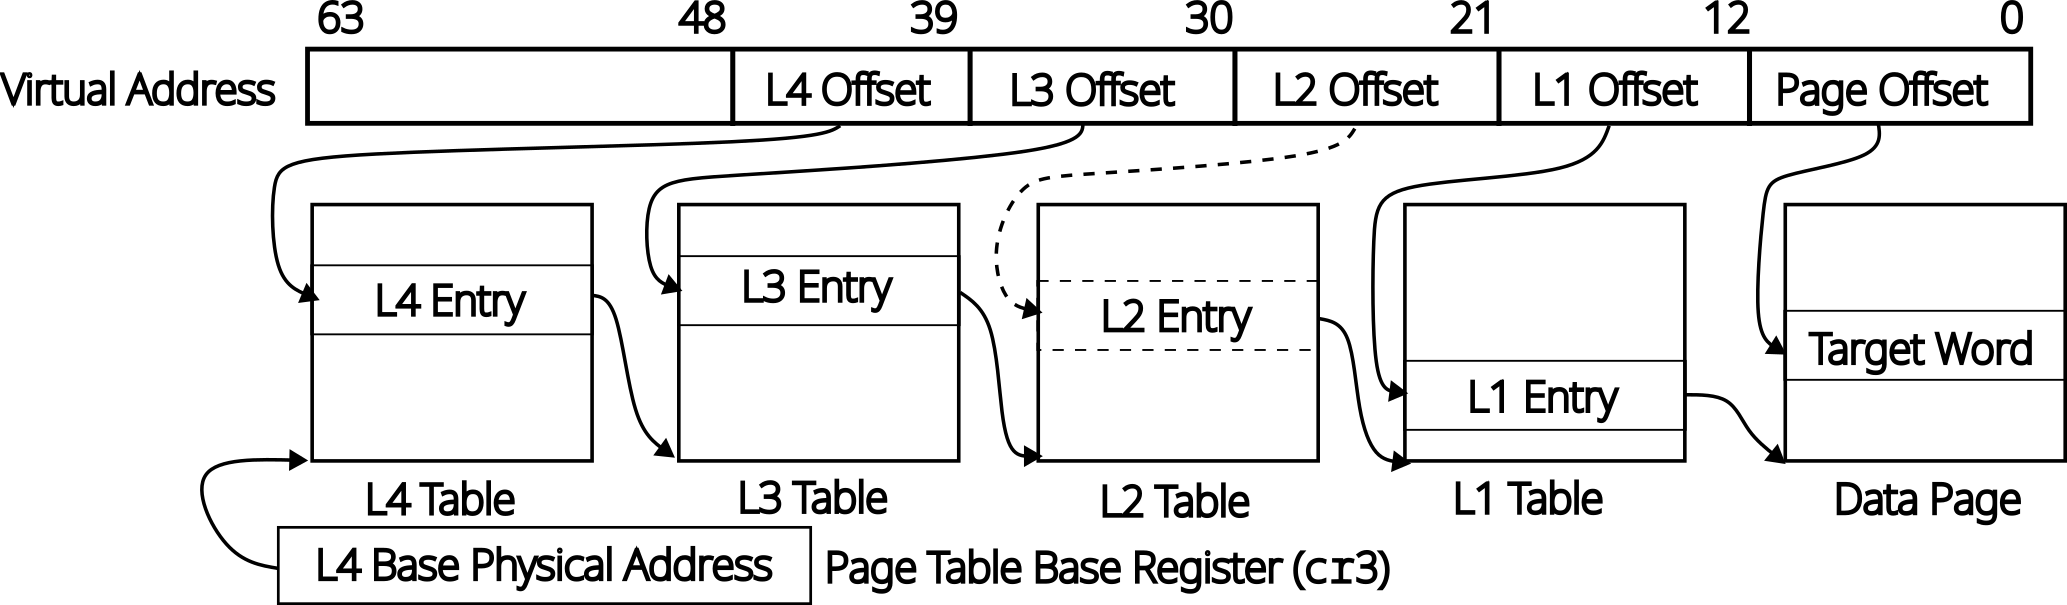
\includegraphics[width=\textwidth]{addr_translation.png}
\vspace{-2em}
          \caption{x86-64 \replace{page table lookups}{hardware address translation}.}
        \label{fig:pagetables}
    \end{subfigure}
    \vfill
\hspace{5em}
\begin{minipage}{.5\textwidth}
%    \begin{figure}
\begin{lstlisting}[mathescape,escapeinside={(*}{*)},basicstyle=\scriptsize]
pte_t *pte_get_next_table(pte_t *entry) {
  pte_t *next;
  if (!entry->present) { // Check if entry needs initialization
    pte_initialize(entry); // Alloc empty table for next level(*\label{line:ptc_alloc}*)
    entry->present = 1; // Mark valid(*\label{line:ptc_mark}*)
  }
  /* Convert phys. addr. from PTE to virt. addr. for access */
  uintptr_t next_phys_addr = PTE_PFN_TO_ADDR(entry->pfn)
  uintptr_t next_virt_addr = (uintptr_t) P2V(next_phys_addr);(*\label{line:ptc_p2v}*)
  next = (pte_t *) next_virt_addr;
  return next;
}
\end{lstlisting}
\end{minipage}
\hfill\hfill
\begin{minipage}{.4\textwidth}
\hspace{3em}
\begin{lstlisting}[mathescape,escapeinside={(*}{*)}, basicstyle=\scriptsize]
pte_t *walkpgdir(pte_t *root, void *va){ 
  pte_t *l4_entry = &root[L4Offset(va)];
  pte_t *l3 = pte_next_table(l4_entry);
  pte_t *l3_entry = &l3[L3Offset(va)];
  pte_t *l2 = pte_next_table(l3_entry);
  pte_t *l2_entry = &l2[L2Offset(va)];  
  pte_t *l1 = pte_next_table(l2_entry);
  pte_t *l1_entry = &l1[L1Offset(va)];  
  return l1_entry
}
\end{lstlisting}
%          \caption{Walking page-table tree to locate L1 entry C-source code.}
%        \label{fig:enter-label}
 %   \end{figure}
\end{minipage}
%\end{framed}
    \vspace{-2.5em}
    \caption{Most of a software page table walk in C, as used to map new pages.}
    \label{fig:pagetablescode}
    \vspace{-1em}
\end{figure}

On the x86-64 architecture, the \textsc{MMU}'s address translation uses a sparse hierarchical set of tables:
\emph{page tables} (referring to pages of memory). As Figure \ref{fig:pagetables} (based on Figure 5-17 of the 
AMD64 architecture manual~\cite{amd64_manual_vol2}\footnote{While x86 up through its 32-bit incarnation were due to Intel,
the x86-64 architecture as a 64-bit extension to x86 was originally due to AMD. As a result, it is sometimes also referred to as the \texttt{amd64} architecture.})
shows,
address translation proceeds by repeatedly taking designated slices of the virtual address and indexing into \replace{a}{successive} table\add{s} \add{of 512 8-byte entries (making each table 4KB in size)}.
The final lookup in the page tables gives the base physical address of a 4KB page of physical memory \add{accessible to the running
program}, to which the low-order
\add{12} bits of the accessed virtual address are added to determine the actual physical address retrieved.
On x86-64, standard configurations use 4 levels of page tables, labelled levels 4 through 1, with lookups in the level 
1 page table resulting in the actual page of physical memory holding the requested data, and the low-order 12 bits 
being used to index into this page.\footnote{Technically levels 1--3 have explicit historical names,
but for brevity and consistency, we simply number them, in keeping with the newer 5th level. Our formalization only deals with 4-level page tables, but is straightforwardly extensible to 5.} 
The translation process or algorithm is \replace{sometimes}{often} referred to as a \emph{page-table walk}.
While Figure \ref{fig:pagetables} and most of our constants (how many levels, which virtual address bits index which
table levels) are specific to \replace{the}{common} x86-64 \replace{architecture}{CPUs},
\replace{
ARMv8 (a.k.a. aarch64), RISC-V, and PowerPC use similar hierarchical page tables for address translation.
RISC-V's sv48 paging configuration~?? and AArch64's 4-level paging configuration
both split 64-bit virtual addresses at the same points to index into the respective tables, so most of what follows
is equally applicable to those architectures (the only difference is that page table entries place control bits of write access, etc.,
in different orders).
}{
  it is straightforward to adapt our approach to ARMv8/\texttt{aarch64}, RISC-V, or PowerPC, which use nearly-identical
  page table structures (only the order of flag bits in the entries differ),
  or to 5-level paging present in newer x86-64 or RISC-V designs (one step would be iterated an additional time).
}

The entries \add{(e.g., L4 Entry in Figure \ref{fig:pagetables})} of each table are 64 bits wide,
but each points to a physical address aligned to 4KB (4096 byte) boundaries, which leaves 12 bits to spare to 
control a validity bit (called the \emph{present} bit), a read-write bit (which permits write access through the entry if and only if it is set),
and a range of additional bits which can be used to control caching, write-through, and more.
This paper will only consider the present bit (0).

The page tables are managed by the \replace{OS, typically by a}{OS kernel's} \emph{virtual memory manager} (VMM).\footnote{Not to be confused with Virtual 
Machine Monitor. We focus on non-hypervisor scenarios, but hardware virtualization extensions for both 
x86-64 and ARM make use of an additional set of page tables translating what a \emph{guest} considers to be its 
(virtualized) physical memory to actual physical memory. Our contributions should offer value in this scenario as well.}
Typically each process has its own 
page tables, which the OS registers with the CPU by storing the (page-aligned)
physical address of the root of the page table tree (the start of the L4 table shown as $\mathsf{root}$ in Figure \ref{fig:pagetables}) in a specific register (\texttt{cr3}) as part of switching to a new process. 
Using different mappings, which map only disjoint portions of physical memory (with some exceptions in the next section) 
is how the OS ensures memory isolation between processes.

If an instruction is executed that accesses a virtual address that either has no mapping, or does not have a mapping permitting 
the kind of access that was performed (e.g., the instruction was a memory write, but the relevant address range was marked read-only in
the relevant page table entry), the hardware triggers a \emph{page fault}, transferring control to a \emph{page fault handler} registered 
with the hardware by the OS, allowing it to take corrective action.
If no mapping was supposed to exist, this is a program bug (e.g., dereferencing virtual address 0 / NULL)
and the faulting program should be terminated. But this can also be used for
\replace{
specialized functionality and optimizations, such as \emph{paging} (saving room in physical RAM and deferring
unnecessary IO by only reading program code from disk when it is accessed, or even swapping memory that has not
recently been accessed to disk, to read back in when a page fault indicates access).
}{
  other purposes such as demand paging to save on IO and better-manage physical memory~\cite{doeppner2010operating}.
}

The key pieces of VMM functionality are
adding a new page mapping (whether the mapped page contains zeros, file data, or swap data), and removing an existing 
page mapping.
While this initially sounds like relatively modest functionality whose implementation may be complicated by hardware 
subtleties, correctness of even these basic operations are actually quite intrictate.
Notably, updates to the page tables are performed as writes to memory --- \emph{which are themselves subject to address translation},
and finding the correct page table to update requires converting between physical and virtual addresses.
In the case of changing the mappings for the currently-active set of page tables, 
\emph{the OS kernel is modifying the tables involved in its
own access of the tables}.
\add{
  To get a sense of how subtle the required reasoning is, we can consider code such as Figure \ref{fig:pagetablescode},
  used in our evaluation to locate the appropriate L1 entry to map a page into the current address space.
  % Adding or removing mappings requires the VMM code to locate the correct page table entry to update,
  % using code such as that in Figure \ref{fig:pagetablescode}.
  \lstinline|walkpgdir| (right) essentially mimics the hardware address translation up to the L1 entry (its caller will modify
  the entry to map a new page),
  indexing into each successive table (e.g., with \lstinline|L4Offset(va)| retrieving the L4 offset of Figure \ref{fig:pagetables}),
  with \lstinline|pte_get_next_table| (left) fetching the base address of the next table
  from each entry.
  If, as shown in Figure \ref{fig:pagetables}, an entry such as the L2 entry is uninitialized (the \emph{present} flag is not set),
  \lstinline|pte_get_next_table| allocates the next table on Line \ref{line:ptc_alloc} and marks it valid on Line \ref{line:ptc_mark}.
  But there is a critical difference from hardware: every memory access in Figure \ref{fig:pagetablescode} uses \emph{virtual} addresses, as opposed
  to hardware's direct physical memory access.
  Thus \lstinline|pte_get_next_table| uses the \lstinline|P2V| (physical-to-virtual) macro on line \ref{line:ptc_p2v}
  to convert physical addresses stored in page table entries into virtual addresses which the kernel can use to access
  the corresponding physical location.
  Proving it correct requires proving that it yields
  an address that is not only mapped, but known to map back to the original physical address!
  Verifying this code is beyond the reach of prior work, which either
  does not model address translation for the kernel~\cite{gu15,gu2018certikos,Klein2009seL4,seL4TOCS,alkassar2008formal}
  and would thus reason unsoundly about this code,
  or models address translation but lacks features required to reason about this code~\cite{kolanski08vstte,kolanski09tphols}.
  We describe our proof of correctness for this code,
  based on the first formalization of critical VMM kernel invariants in an MMU-aware logic, in Section \ref{sec:experiment}.
}
\looseness=-1


Virtual memory concerns propagate to the OS scheduler, which deals with multiple 
address spaces, so must keep track of which virtual addresses are valid (and in what way) in which address spaces. 
Some virtual addresses are valid in only a single address space (e.g., a code address for a particular usermode 
process), while others are valid in all address spaces (e.g., kernel data structure pointers). 
The VMM must maintain some of these assumptions on behalf of the rest of the kernel, for example by guaranteeing that 
a certain range of virtual addresses (corresponding to the kernel's code and data) are valid in every address space.

% \paragraph{\add{Mapping a New Page}}
% \add{Mapping a new page into a virtual address space is a key piece fo functionality, and also a key challenge for verification.
% This operation takes a chunk of physical memory to install, and a (page-aligned) virtual address at which to make it
% visible to the process.
% Starting from the page table root (\lstinline|cr3| in Figure \ref{fig:pagetables}), it must traverse the page tables until it locates
% the correct location of the L1 entry which should point to the physical page (installing new L3, L2, and L1 tables as needed),
% and update the L1 entry to point to the physical page. This is complicated by the fact that the kernel accesses the page
% tables through \emph{virtual} addresses, but the page table root and the addresses in the L4--L1 entries are all \emph{physical}
% addresses. So the mapping process must repeatedly perform \emph{backwards} mappings (not supported by hardware) from
% physical addresses of each level's entry to a virtual address that is then mapped back to the corresponding physical address!
% And for modularity, the translation process (and possible allocation of missing tables) is typically implemented in a function
% used for every level of translation (i.e., a level-polymorphic function).
% These compounding subtleties are one reason \textsc{CertiKOS} and \textsc{seL4} \emph{trust} their page table
% manipulations; both the reasoning to prove correctness, and the kernel invariants that ensure correctness of typical implementations,
% are remarkably subtle.
% }
% \looseness=-1

\paragraph{Out of Scope: Translation Lookaside Buffers (TLBs)}
CPUs with MMUs typically have an additional \emph{translation lookaside buffer}
(TLB), to cache the (successful) results of page table walks, rather than transforming every virtual
memory access into 5 physical accesses. 
Any time a virtual address that was accessible becomes inaccessible (or has downgraded permissions),
the TLB (or at least entries in affected virtual address ranges) should be flushed.
In most kernels, this occurs in only a few well-known places, which is why existing verified kernels
\textsc{seL4}~\cite{Klein2009seL4,seL4TOCS} and \textsc{CertiKOS}~\cite{gu15,gu2016certikos} currently
trust that TLB flushes are handled correctly rather than actually modeling TLB hardware and verifying.
Eventual verification of TLB handling is a worthwhile long-term goal, but it is a challenging pursuit in its
own right. Based on others' early progress on verifying TLB operations in isolation~\cite{syeda2020formal}, we expect
it to be possible to combine this paper's insights with that support. 
Section \ref{sec:relwork} elaborates briefly on the challenges involved.
Even without TLB modeling,
our logic already enables verification of virtual memory management functionality that prior verified kernel work
either trusts completely (\textsc{seL4}, \textsc{CertiKOS}) or is incapable of reasoning about.
% Appendix \ref{apdx:tlb} gives more details on the challenges involved for the interested reader.
\looseness=-1

% \subsection{Virtual Memory Managers}
% \label{sec:backgroundonvmm}
% Most OS kernels have a component called a \emph{Virtual Memory Manager} (VMM)
% which is responsible for setting up page table mappings and for taking action when a page fault occurs. Often, a page 
% fault indicates a bug in a program --- for example, a null pointer dereference crashes a program not because the hardware
%  designates it an error, but because most OSes refuse to map the first 4K worth of virtual addresses, so dereferencing 
% \texttt{NULL} results in a page fault. In such cases, the OS will terminate the program.

% In other cases the OS uses page faults to implement specialized functionality and optimizations. A key example of this is 
% (confusingly) called \emph{paging}: saving room in physical RAM and avoiding unnecessary IO 
% by waiting until memory addresses for code are accessed 
% before copying them to RAM (in particular, saving process startup time); 
% or copying memory that has not recently been accessed to disk 
% (i.e., in a \emph{swap} file or partition) and marking those page table entries invalid so a future page fault will give 
% the OS the chance to copy the relevant data back into memory when the program tries to access it again.


% \todo[inline]{Colin says: we should chat about the paragraph below. We don't want to advertise too many
% challenges of VMM verification that we don't actually solve (or rather, we'd push them to the and of the paper
% as future work). But some of these I think we could split the difference with, for example by defining
% a variant of virtual-pointsto that allowed virtual address aliasing, but not actually verifying any code examples
% with it (just showing it's compatible with our approach).
% }
% For one, virtual addresses may \emph{alias} when more than one is mapped to the same physical memory. 
% This can occur when a process requests it (e.g., via \texttt{mmap} or \texttt{shm\_open} on UNIX-style kernels). 
% It also occurs automatically in most general-purpose kernels: while for normal programs the OS uses the MMU to isolate 
% and abstract physical memory, the kernel's own functionality is often easier to implement if the kernel can directly 
% access memory given its physical address, for example when interacting with hardware devices. For this reason, most 
% kernels contain an \emph{identity map} of all physical memory in a machine. 
% \todo[inline]{We should try defining an identity map on a whiteboard and see what breaks. If it's feasible we should
% tweak and get a definition in the paper. If not, we should cut the identity map discussion.}
% In some cases this is a literal identity map, 
% where for every virtual address $p$, interpreting $p$ as a virtual address instead will map back to $p$ as a physical 
% address. In other cases there is an offset involved, where to access physical address $p$ the kernel can access virtual
%  address $p+\mathit{offset}$. This identity map saves the kernel the performance cost of having to continually add and
%  remove transient mappings simply to briefly access a specific physical memory region. But this coexists with additional
%  virtual addresses (those used by most kernel code and data structures), in a form of virtual address aliasing. Note 
% that virtual address aliasing is both prevalent in general-purpose kernels, and violates the core assumption of most 
% memory models assumed by verified compilers like CompCert, which assume no virtual address aliasing.

% \todo[inline]{Colin says: Again, let's chat about the next paragraph. This might be another where we can
% split the difference on extension by defining something and proving a $\ast-\ast$ kind of result for sharing
% page table fragments, rather than actually proving any new code. I'm less sure about this one, though.
% }
% Another complicating factor is that portions of page tables can be shared, i.e., trees of page tables can overlap and
% become forests. 
% One common way this used to happen was for one subtree of page tables to map the kernel if linked in appropriately to 
% a higher-level page table, and then to reuse that kernel mapping portion in every process's page tables. This was mostly 
% phased out in the wake of Spectre, but remains relevant on correctly-implemented hardware.

\subsection{Separation Logic}
\label{sec:seplogic}
% \todo{Colin says: I added this b/c prior systems reviewers wanted more verification background...
% not sure how I feel about it}
Separation logic~\cite{reynolds02} is a descendant of classic Hoare logic~\cite{hoare69},
where in addition to pre- and postcondition assertions, assertions themselves pick up a
\emph{separating conjunction} operator $\ast$, such that an assertion $A\ast B$ means $A$ and $B$ are true
of disjoint pieces of state. This allows for local reasoning about updates, because it articulates
that updates to the state backing $A$ do not affect the truth of $B$. This is classically demonstrated
through the \emph{points-to} assertion: $l\mapsto v$ asserts that the memory cell at address $l$ holds value $v$:
knowing $x\mapsto 3\ast y\mapsto 4$ and writing through $x$ means information about $y$ is preserved:
$\{x\mapsto 3\ast P\}\;x\mathrel{:=}5\;\{x\mapsto 5 \ast P\}$ can be derived for any $P$.

We build on the \iris~\cite{jung2018iris} separation logic framework,
an abstract separation logic embedded in Rocq, which is useful for both metatheoretical work
and interactive correctness proofs using the logic. Given an operational
semantics structured a certain way (in our case, semantics for
a fragment of x86-64 assembly including address translation),
if a small number of ``glue'' lemmas are proven, \iris
provides a ready-made separation logic with a number of advanced features, including
higher-order ghost state and impredicative invariants, for no additional work.

We suppress \replace{many details of Iris assertions}{some technical \iris details} for brevity, but briefly note
a few recurring details used heavily in \iris but not necessarily in traditional
separation logics.
Because \iris is an embedded framework in \rocq, proofs in \iris-derived
logics often encapsulate raw \rocq assertions: $\ulcorner P \urcorner$ is an embedding
of the \rocq assertion $P$ into an \iris assertion (used for things like equality and other
general pure logical assertions), similar to prior \rocq-embedded program logics~\cite{Chlipala2013Bedrock}. Newly-defined \iris assertions are in fact
\rocq terms of a particular type, rather than being drawn from a fixed vocabulary.
\looseness=-1

\iris includes two forms of implication. The magic wand operator $\wand$ is an affine implication:
$A\wand B$ describes a resource which, if combined with a resource satisfying $A$, will satisfy $B$.
Notably, this implication involves no changes to ghost state. \iris, building on the Views framework~\cite{Dinsdale-Young2013Views},
also includes a \emph{view shift} operator $\vs$ which models updates to ghost state: $A \vs B$
means resources satisfying $A$ may be transformed into resources satisfying $B$, intuitively by updating only ghost state.\footnote{\iris
experts may note that this is \emph{technically} mildly misleading given how \iris's update modalities and weakest precondition
are defined, but
this is adequate intuition for non-experts in \iris to follow their use.
}
View shifts are essentially logical entailment plus ghost updates.
\looseness=-1

% Of particular interest to us, \iris's machinery is largely agnostic to the particular choice of
% \emph{resource algebra}\footnote{A modern descendant of the venerable partial commutative monoid used
% to abstractly model earlier separation logics~\cite{calcagno2007local}, 
% with additions to support the step-indexing required to solve the recursive domain equations
% that arise with higher-order ghost state and impredicativity~\cite{birkedal2011step,hobor2010theory}.
% }
% used to give algebraic semantics to the connectives of the assertion language.
% This means we can drop in an alternative model that naturally supports working with respect to
% a locally-fixed context, like an address space.

% Also relevant is that \textsc{Iris} naturally decomposes the traditional Hoare triple $\{P\}\;C\;\{Q\}$
% into the precondition implying the weakest precondition of the program with respect to the postcondition ---
% $P \wand \textsf{wp}\;C\;\{v\ldotp Q\}$.\footnote{An idea with long history~\cite{pratt1976semantical}.}
% This is a natural fit for assembly-level verification, where the \emph{Hoare double}

An important limitation is that to date, every separation logic
has assumed that all pointer addresses are meant for use in a single address space, which avoided the
problem of tracking that certain points-to assertions are true only for certain address spaces, but not others.

\subsection{Modal Logic}
\label{sec:backgroundonmodallogic}
The problem of needing to keep track of things being true in some contexts and not in others is hardly unique to virtual 
memory management, and is the general insight behind most flavors of modal logic, which use
unary operators to express that a logical claim $P$ is \emph{contingently} true 
in certain other circumstances, such as in other times~\cite{pnueli1977temporal} or places~\cite{murphy2008type,gordon2019modal}.

%   A unifying concept across any modality is that they behave as applicative functors, 
% typically satisfying (directly, or as a derived law, depending on the modality):
% \[ (P\rightarrow Q) \rightarrow M(P) \rightarrow M(Q)\]
% %\todo[inline]{Ismail, I think this means we have pure intro, $\square P \mathrel{-\ast} [r](\square P)$ if I'm using the right symbol for pure assertions }
% %\todo[inline,color=red]{The above todo comment isn't quite right.
% %Purity is about being able to duplicate. You had defined another typeclass/property-of-assertions that meant it didn't
% %care what address space it was in (like physical pointstos). That's orthogonal to purity.
% %}
% Many modalities, so-called \emph{normal} modalities also possess introduction rules of the form $P\rightarrow M(P)$, 
% the classic example being that if $P$ is true, then $P$ is \emph{necessarily} true with the contingency picked up.%($\square P$).

Of particular interest for reasoning about virtual memory are modalities that permit \emph{naming} the alternate 
circumstances, prominently \emph{hybrid} modal logics~\cite{blackburn1995hybrid,areces2001hybrid}, which come equipped 
with assertions of the form $[\ell](P)$ indicating that $P$ is true in the specific alternate circumstance (Kripke world)
 named by the \replace{\emph{nominal}}{term} $\ell$. Note that a distinctive property of hybrid logics is that, rather than hiding
the points at which a modal assertion is evaluated inside the modality's definition, the choice of what world a modalized
assertion should be true in is chosen \emph{in the assertion itself}. This allows assertions to talk about not simply whether some other assertion
is true in some possible future or past world related in a fixed way to the current world, but to talk about \emph{arbitrary}
other worlds.
\add{This is somewhat different from the accessibility relation modalities more common in verification, but also well-established,
tracing its origin back to Arthur Prior~\cite{areces2006hybrid}, just as many temporal logics do.}

This explicit naming of alternate worlds increases the power of \add{propositional} modal logics~\cite{blackburn1995hybrid}, and is 
necessary for completeness in classical separation logics~\cite{brotherston2014parametric}.
\add{However typically modal logics can always be ``compiled'' into logics with suitable quantifiers:
the \emph{standard translation}~\cite{blackburn2006modal} of propositional modal logics into first-order logic
has been thoroughly studied. \textsc{Iris}'s support for higher-order impredicative quantification means
this applies to our modalities as well --- they do not strictly speaking make \textsc{Iris} more expressive.
But while propositional modal logics are no more expressive than first-order logic (with just two variables!),
the primary goal of a modal logic is not raw expressive power but intuitive specifications and proof rules.
Temporal logics are used because they simplify specifications (vs. having explicit time variables
in every base asertion) and reasoning principles (because the modal correspondents of quantification over
time is used in a highly structured way).
Our logic offers a similar value proposition: natural specifications and reasoning principles which
are powerful enough for reasoning about virtual memory management, but without requiring pervasive tracking of
and explicit abstraction over address spaces.
}


For our purposes, these are natural candidates to adapt for virtual memory management. We can reinterpret the notion of 
naming an alternate world slightly more loosely, and instead name \emph{address spaces} by the physical address of the 
page table root, since these structures are the physical representations of page tables. Thus in this paper we develop 
the notion that we can represent contingent truth of an assertion via $[r](P)$ indicating that $P$ holds in the address 
space rooted at physical address $r$. Because OS kernels create and destroy address spaces, it is sensible to use
a hybrid-style logic that is not specialized to a fixed set of modalities, but this introduces
some subtleties from the fact that the existence of certain modalities (address spaces) can change.


% The typical hybrid modality introduction rule, that $P$ and $\ell$ (indicating the current world is $\ell$) imply 
% $[\ell](P)$, has a natural analogue: knowing $P$ and that the current address space is $r$ (i.e., that $r$ is the 
% current \texttt{cr3} value) suggests a way to construct $[r](P)$. 
% We identify an assertion as \emph{contextual} if its validity depends on the choice of address space. Used outside an explicit
% modality, the truth of this assertion depends on the current \texttt{cr3} value. Used under an explicit address space
% modality, its truth depends on both the modality-chosen address space and associated physical resources.
% \begin{itemize}
%   \item as a \textit{contextual} fact if its validity depends on \texttt{cr3} when it is outside the modality (i.e. modal context), and made 
%   \texttt{cr3} independent as a part of custom-tailored modal logic for virtual-memory: a truth representing a virtual-memory addressing depends
%    \texttt{cr3} due to address-translation operation, is dependent on \texttt{cr3} in the ambient-logic (e.g. separation-logic),
%     and is made \textit{independent} of the facts related to \texttt{cr3} by being introduced into the modal context under the assumption that
%     it exhibits the knowledge on its validity with respect to \texttt{cr3} in the ambient logic.
%   \item as a \textit{pure} fact as long as it does not \textit{necessarily} depend on any fact related to \texttt{cr3}: a truth representing a raw physical memory addressing, unlike virtual-address translation, does not need the \textit{knowledge} of \texttt{cr3}, therefore it can be introduce into the modal context as a pure fact
% \end{itemize}

Interaction of hybrid modalities and substructural reasoning is relatively unexplored (see Section \ref{sec:relwork}).
% A relatively under-explored space of modal logics is the interaction of modal and substructural logics, 
% in particular hybrid-style modalities in substructural logics, which has seen only minimal exploration~\cite{dovsen1992modal,restall1993modalities,d1997grafting,kamide2002kripke,licata2017fibrational} and no prior 
% application. 
Our development atop \iris~\cite{jung2018iris} needs to explore some additional subtleties 
that arise where the modality itself may entail ownership of resources, 
as well as interactions between our hybrid-style 
modality and substructural rules.  
% For example, Iris contains a number of modalities that distribute over separating 
% conjunction, or for which resources can freely move into the modality 
% (e.g., $\blacktriangleright(P)\ast Q \wand \blacktriangleright(P\ast Q)$). In our setting some of these rules 
% apply while others do not. For example, 
% In our setting, an assertion that involves no modalities is interpreted as 
% holding in the current (active-on-the-CPU) address space, so clearly cannot move into arbitrary other address spaces,
% while address-space-relative assertions 
% --- unless guarded by another address space modality.
Some prior \iris-based work~\cite{dang2019rustbelt,dang2022compass} has constructed derived modalities in the style we propose, indexed
by thread IDs. However \replace{in that setting, the}{their} intepretation of those modalities was fully fixed ahead of time (to refer to essentially buffers in operationalized versions of C11
concurrency). In this setting, while our modalities will be indexed by page table roots, it is possible to modify the address translation for an address
space with root $r$ --- thus changing the interpretation of a modality, and even whether a modality is valid --- \emph{while assertions with that modality are active}.
\add{This is essential to updating page mappings for the current address space in use by a CPU.}
\looseness=-1
